\chapter{Girth, ordering and coloring of hypergraphs}

\section{Size of edges -- lemma}

For simple $k$-graphs $(X, \M)$ we have shown that $\chi$ may be unbounded, due to Ramsey and Hales Jewett, but $PG(g)$ has $\chi = 2$ for $g > 2$. Also $\M \sim \binom{|X|}{2}$ due to Erd\H os and Hanani. Now lets see if $|\M| \geq |X|^{1 + \epsilon}$ can be true. Before showing the proof lets show some direct results from such statement.

\begin{thm}[Ordering property]
	Assume $|\M| \geq |X|^{1 + \epsilon}$ fo given $k, \epsilon$ and large $X$. $\forall G = (V,E)$ and $\forall$ linear ordering of $V$ there exists graph $H = (W,F)$ such that for every linear ordering $\preceq$ of $W$ there exist monotone embedding $f : (G, \leq) \to (H, \preceq)$. In particular $f : V \to W$, $\{x,y\} \in E \iff \{f(x), f(y)\} \in F$ and $x \leq y \iff f(x) \preceq f(y)$.
\end{thm}

\begin{proof}
	Let $G = (V,E)$ be given and $|V| = k$. Let $(X, \M)$ be simple $k$-graph with $n$ vertices. Let $\mathcal{G}$ be the set of all graphs $H = (X,F)$ with property that for any $M \in \M$ the graph $H|_M \simeq G$ and every edge of $F$ is a subset of an $M \in \M$. Then the number of placements of different orderings of $G$ is $a = \frac{k!}{\mathtt{Aut}(G)}$ where $\mathtt{Aut}(G)$ is the automorfism group of graph $G$.
	
	Then $|\mathcal{G}| = a^{|\M|} \geq a^{n^{1+\epsilon}}$. How many graphs $H$ in $\mathcal{G}$ contain embedding $(G, \leq) \to (H, \preceq)$ for some $\preceq$? That is $\leq n! (a - 1)^{n^{1+\epsilon}}$ which is $\ll a^{n^{1+\epsilon}}$, which can be seen by taking logarithms.
	
	$$
	n^{1 + \epsilon} \log a > n \log n + n^{1 + \epsilon} \log(a-1)
	$$
	
	\noindent Hence there exists $H \in \mathcal{G}$ such that it suffices the property.
\end{proof}

Other remark is that there exists $H$ where all orderings of $(G, \leq)$ appear almost equally likely, which was shown by Angel, Kechris and Lyons. The technique is called \textit{random placement method} used in 1991 by Nešetřil, Rodl and Ramsey.

Now we will show a stronger version of our stated property.

\begin{thm}
	$\forall k \ \forall l \ \exists \epsilon$ there exist $(X, \M)$ $k$-graph such that
	
	\begin{enumerate}
		\item $|\M| \geq |X|^{1 + \epsilon}$ and
		\item $(X, \M)$ has no cycles of length $\leq l$.
	\end{enumerate}
	\label{big-sized-k-graph}
\end{thm}

Note that we can have cycles of length $2$ by just having $M \neq M' \in \M$ where $|M \cap M'| = 2$. This can be seen by drawing the incidence bipartite graph, where we have cycles of length $2l$ in comparison to the circles inside a $k$-graph. Hence for $l = 3$ we obtain the original statement.

\begin{proof}{Proof with stronger theorem.}
	Let $G = (V,E)$ be given and $|V| = k$. Let $(X, \M)$ be simple $k$-graph with $n$ vertices. Let $\mathcal{G}$ be the set of all graphs $H = (X,F)$ with property that for any $M \in \M$ the graph $H|_M \simeq G$ and every edge of $F$ is a subset of an $M \in \M$. Also $H$ contains cycles of length $\leq l$ only in copies of $G$.
\end{proof}

\begin{thm}
	$\forall k \ \forall l \ \exists G_{k,l} = G$:
	
	\begin{enumerate}
		\item $\chi(G) \geq k$ and
		\item $G$ contains no cycles $C_3, C_4, \dots, C_{l-1}$.
	\end{enumerate}
\end{thm}

\begin{proof}
	Put $K = k+1$ and apply stronger theorem \ref{big-sized-k-graph} for $K,l$, then we get $(X, \M)$ $K$-graph and $|X| = n$ and $|\M| \geq |X|^{1 + \epsilon}$. We take $M \in \M$ and we put there one edge. $\mathcal{G} = \{(X,E); (X,E)|_M \simeq \text{only one edge}\}$.
	
	Now $a = \binom{K}{2}$ and any $H \in \mathcal{G}$ does not contain short cycles. How many graphs $H$ in $\mathcal{G}$ have a $\chi(H) \leq k$?
	
	So $\exists f: X \to \{1, 2, \dots, k\}$ on every $M \in \M$ $\exists x \neq y$ such that $f(x) \neq f(y)$. $|\mathcal{G}| = a^{n^{1+\epsilon}} \gg |\{G | \chi(G) \leq k, G \in \mathcal{G}\}| = k^n \cdot (a-1)^{n^{1 + \epsilon}}$.
\end{proof}

Now suppose we have a poset $P = (X, \leq)$ and we create Hase diagram. Question: Which graphs are diagrams? For planar graphs it holds that $G$ is diagram $\iff K_{3} \nsubseteq G \Rightarrow \chi(G) \leq 3$. Problem is that whether there exists graph without $C$ of length $[3, l]$ which fails to be a diagram? Then there is a theorem which states that indeed it is true for all $l$. $G$ is not a diagram $\iff \forall$ ordering $\leq$ of $V(G)$ there exists a cycle of length $t$ for some $t$.

\begin{proof}{Proof of theorem \ref{big-sized-k-graph}}
	Set $\epsilon = \frac{1}{l}$ and put $m = 2 \cdot n^{1+\epsilon}$. Consider all $k$-graphs with $m$ edges and $n$ vertices. There is exactly $\binom{\binom{n}{k}}{m}$ such $k$-graphs. Observe that if $(X, \M)$ has no cycles then $|\M| (k - 1) + 1 \leq |X|$. How many of these $k$-graphs contain a cycle of length $l' \leq l$? By this observation it must be violated so it must be
	
	$$
	\leq c(k, l') n^{(k-1)l'} \binom{\binom{n}{k} - l'}{m - l'}
	$$
	
	\noindent where
	
	$$
	c(k, l') = \binom{\binom{l'(l-1)}{k}}{l'}.
	$$
	
	Lets divide it be $\binom{\binom{n}{k}}{m}$ which leads to upper bound for average number of cycles of length $l'$. So we proceed by summing it over all $l' \leq l$.  Obtaining the following.
	
	$$
	\sum_{l' \leq l} \frac{c(k, l') n^{(k-1)l'} \binom{\binom{n}{k} - l'}{m - l'}}{\binom{\binom{n}{k}}{m}}
	$$
	
	We can simplify the binomials and just obtain
	
	$$
	\frac{m \cdot (m - 1) \cdots 2 \cdot 1}{\binom{n}{k} \cdot (\binom{n}{k} - 1) \cdots (\binom{n}{k} - l' + 1)} \cdot n^{kl' - l'}
	$$
	
	\noindent and we are considering only with going to $\infty$, that is the leading elements of such polynomials. Hence we have
	
	$$
	\leq c \cdot n^{kl' - l'} \cdot \frac{m^{l'}}{n^{kl'}} = c \cdot n^{-l'} \cdot n^{(1 + \epsilon) l'} = c \cdot n^{\epsilon l'} \leq n \cdot c.
	$$
	
	Therefore there has to be $k$-graph with such small number of short cycles. For that we will delete at most $cn$ edges to get rid of every short cycle.
\end{proof}

Note that for this theorem there does not exist a constructive proof.

\begin{cor}
	$\forall p, k \geq 2, l \geq 2$ $\exists (Y, \mathcal{N})$ such that
	
	\begin{enumerate}
		\item $\mathcal{N} \subseteq \binom{Y}{k}$,
		\item $(Y, \mathcal{N})$ has girth $> l$ and
		\item $\chi(Y, \mathcal{N}) > p$.
	\end{enumerate}
	\label{chromatic-girth}
\end{cor}

\begin{proof}
	Put $K = p (k-1) + 1$ and let $(X, \M)$ be simple hypergraph such that $\M \subseteq \binom{X}{K}$ and $(X, \M)$ has girth $> l$ and $|\M| \geq |X|^{1+\epsilon}$ (by using the theorem \ref{big-sized-k-graph}). Let $\mathcal{H}$ be the set of all graphs $(X, \mathcal{N})$, where $\mathcal{N} \subseteq \binom{X}{k}$ such that
	
	\begin{enumerate}
		\item for every $M \in \M$ there exists $\leq 1$ $N \in \mathcal{N}$ where $N \subseteq M$ and
		\item there are no other edges.
	\end{enumerate}
	
	\noindent Any $(X, \mathcal{N}) \in \mathcal{H}$ has girth $> l$. How many $k$-graphs from $\mathcal{H}$ have a chromatic number $< p$? That would be
	
	$$
	\leq p^{|X|} \cdot \left(\binom{K}{k} - 1\right)^{|X|^{1 + \epsilon}}
	$$
	
	\noindent since it is the number of colorings multiplied by the number of $k$-graphs with given coloring (respectively). This is
	
	$$
	\ll |\mathcal{H}| = \left(\binom{K}{k}\right)^{|X|^{1 + \epsilon}}.
	$$
\end{proof}

We will also present a constructive proof in this case. But before we do so, we state some remarks. Usually the \textit{chromatic number} of a graphs is something like the complexity, or in other words it cannot be split into small pieces. On the other hand \textit{girth} is something like local simplicity. So the theorem states that even a graph which locally seems simple it is still complex.

\section{Unavoidable configurations}

\begin{defn}
	Graph $F$ is $\chi$-unavoidable if $\exists n_0(F)$ for every graph $G$ with $\chi(G) \geq n_0(F)$ contains $F$ as a subgraph (not necessarily induced).
\end{defn}

\begin{cor}
	Forests are only $\chi$-unavoidable graphs.
\end{cor}

\begin{proof}
	If $F$ is not a forest then $F$ has a cycle of length $l$ which by using the theorem \ref{chromatic-girth} can be still made arbitrarily colourful.
	
	Suppose $\chi(G) \gg n_0$ and $F$ is a tree. This implies that $\Delta(G) > n_0$, where $\Delta(G)$ denotes the maximum degree.
	
	Lets have vertices with small degrees and then delete them. Now we may end up with other vertices which now have small degree so we proceed in the same way until we can. After that we take a vertex with the maximum degree this has to have other vertices which also have a high degree and so on, this is how the tree can be constructed.
\end{proof}

\begin{cor}
	$\forall k \ \forall F$ $K$-graph tree $\exists n_0(k,F)$ such that any $\chi(X, \M) \geq n_0$ contains $F$.
\end{cor}

\begin{lemma}
	Any $k$-graph with high chromatic number contains large degree. (Sometimes this is called a sunflower or $\Delta$ system).
\end{lemma}

\begin{proof}
	Suppose $\chi(X, \M) \geq (k-1) \cdot t = n_0$. Then we split vertices into a groups $X_1, X_2, \dots, X_{n_0}$ by their colours. We will take $X_1$ and enlarge it to $X_1'$ as much as possible without violating the colouring. Then for $X_2$ we take $X_2' = X_2 \setminus X_1'$ and again enlarge it. We will continue with all groups. All of them have to be non-empty, otherwise the colouring was not optimal. Lets have $x \in X_{n_0}'$. There has to be an edge to $X_1', X_2', \dots$, because otherwise we would add $x$ to one of them. This is how we got our sunflower.
\end{proof}

\begin{conj}
	Any high chromatic graphs contains either large $K_n$ or given induced tree $T$. Alternatively: Fix $T$ tree, $K_n$. Let $G$ be a graph $K_n \nsubseteq G$ and $T \not\sqsubseteq G$ then $\chi(G) \leq n_0(T, K_n)$.
\end{conj}

\begin{conj}
	Same statement is not true for $k$-graphs.
\end{conj}

\begin{example}
	Lets consider $k = 2$ so graphs and $l = 4$, therefore triangle-free graphs. Try to create $\forall n$ a graph such that $C_3 \nsubseteq G$ and $\chi(G) = n$. For $n = 3$ we take an odd cycle of length 5. Now we can proceed by Mycielski and construct this graph \ref{mycielski}
	
	\begin{figure}[!ht]\centering
		\begin{subfigure}{.45\textwidth}\centering
			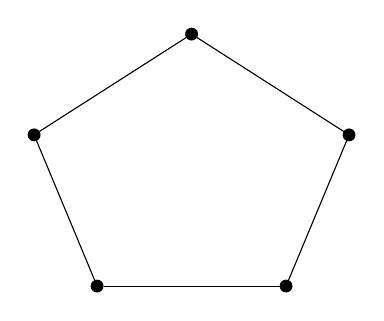
\begin{tikzpicture}[n/.style = {draw, circle, fill, inner sep=1.5pt}, scale=.8]
				\node[n] (0) at (0,0) {};
				\node[n] (1) at (3,0) {};
				\node[n] (2) at (-1,2.4) {};
				\node[n] (3) at (4,2.4) {};
				\node[n] (4) at (1.5,4) {};
				
				\draw (0) -- (1);
				\draw (0) -- (2);
				\draw (3) -- (1);
				\draw (3) -- (4);
				\draw (2) -- (4);
			\end{tikzpicture}
			\caption{Five cycle.}
		\end{subfigure}
		\begin{subfigure}{.45\textwidth}\centering
			\begin{tikzpicture}[n/.style = {draw, circle, fill, inner sep=1.5pt}, scale=.8, b/.style = {myblue, line width=1pt}]
				\node[n] (0) at (0,0) {};
				\node[n] (1) at (3,0) {};
				\node[n] (2) at (-1,2.4) {};
				\node[n] (3) at (4,2.4) {};
				\node[n] (4) at (1.5,4) {};
				
				\node[n,b] (0b) at (0.6,0.6) {};
				\node[n,b] (1b) at (2.4,0.6) {};
				\node[n,b] (2b) at (-0.4,2.4) {};
				\node[n,b] (3b) at (3.4,2.4) {};
				\node[n,b] (4b) at (1.5,3.4) {};
				
				\node[n,b] (c) at (1.5, 2) {};
				
				\draw (0) -- (1);
				\draw (0) -- (2);
				\draw (3) -- (1);
				\draw (3) -- (4);
				\draw (2) -- (4);
				
				\draw[b] (0b) -- (1);
				\draw[b] (0b) -- (2);
				\draw[b] (3b) -- (1);
				\draw[b] (3b) -- (4);
				\draw[b] (2b) -- (4);
				\draw[b] (0) -- (1b);
				\draw[b] (0) -- (2b);
				\draw[b] (3) -- (1b);
				\draw[b] (3) -- (4b);
				\draw[b] (2) -- (4b);
				
				\draw[b] (c) -- (1b);
				\draw[b] (c) -- (2b);
				\draw[b] (c) -- (3b);
				\draw[b] (c) -- (4b);
				\draw[b] (c) -- (0b);
			\end{tikzpicture}
			\caption{Adding brothers and common point.}
		\end{subfigure}
		\caption{Mycielski creation of a graph.}
		\label{mycielski}
	\end{figure}
	
	This can be actually generalized. Lets have $G_n$, for every vertex of such graph create a \textit{"brother"} which will share the same neighbours. Then also create one common vertex and connect all \textit{brothers} to him. See that this has chromatic number at least $n+1$ if $G_n$ had chromatic at least $n$.
\end{example}

\begin{example}
	Another construction is so called \textit{Shift graph.} We will create $G_n$ by taking $V$ to be $E(K_n)$ and $E(G_n)$ being two consecutive edges in $K_n$ by an ordering $\leq$. This graph also does not have triangles and $\chi(G_n) = \log n$. Suppose that $\chi(G_n) \leq t$ then $E = E_1 \dot\cup E_2 \dot\cup \dots \dot\cup E_t = E(K_n)$ easily seen that $\chi([n], E_i) \leq 2$ since no beginnings and ends can overlap. Therefore $\chi(K_n) \leq 2^t$, where the logarithm follows.
\end{example}

\section{Constructions}

\begin{thm}
	$\forall u,g,r$ there exists an $u$-uniform hypergraph of girth $\geq g$ and chromatic number $\geq r$.
\end{thm}

\begin{defn}
	$n$-partite uniform hypergraph is $(V_1, \dots, V_n, E)$ where $E \subseteq \binom{V_1 \cup \dots \cup V_n}{u}$ and $V_1, \dots, V_n$ are pairwise disjoint and $\forall e \in E \ \forall i < n \ |e \cap V_i| \leq 1$. 
\end{defn}

\begin{example}
	For example if we set $u = 2$ and $n = 2$ then we obtain normal bipartite graph.
\end{example}

\begin{proof}[By partite construction -- Nešetřil and Rodl]
	We will se a proof for $g = 4$ and every $u,r$. Let $N \to (u)_r^1$ be pigeon hole number $N = (u-1) \cdot r + 1$. Picture 0 is $N$-partite hypergraph created as a disjoint union of $\binom{N}{u}$. Edges are one for every projections.
	
	\begin{figure}[!ht]\centering
		\begin{tikzpicture}[main/.style = {draw, circle, inner sep=2.5pt}]
			\node[main] at (0,3) {$P_0^1$};
			\node[main] at (0,2) {$P_0^2$};
			\node[main] at (0,1) {$P_0^3$};
			\node[main] at (0,0) {$P_0^4$};
			\draw (1,3) -- (8,3);
			\draw (1,2) -- (8,2);
			\draw (1,1) -- (8,1);
			\draw (1,0) -- (8,0);
			\node[main, myorange, fill] (1) at (2,3) {};
			\node[main, mygreen, fill] (2) at (2,2) {};
			\node[main, mygreen, fill] (3) at (3,2) {};
			\node[main, myorange, fill] (4) at (3,1) {};
			\node[main, myorange, fill] (5) at (4,1) {};
			\node[main, myblue, fill] (6) at (4,0) {};
			\node[main, myorange, fill] (7) at (5,3) {};
			\node[main, myorange, fill] (8) at (5,1) {};
			\node[main, mygreen, fill] (9) at (6,2) {};
			\node[main, myblue, fill] (10) at (6,0) {};
			\node[main, myorange, fill] (11) at (7,3) {};
			\node[main, myblue, fill] (12) at (7,0) {};
			\draw (1) -- (2);
			\draw (3) -- (4);
			\draw (5) -- (6);
			\draw (7) -- (8);
			\draw (9) -- (10);
			\draw (11) -- (12);
		\end{tikzpicture}
		\caption{Example: Picture 0 for $u = 2, r =3$ and hence $N = 4$ with nice coloring having a monochromatic edge.}
	\end{figure}

	Observe that if picture 0 is $r$-colored such that vertices with the same projection has the same color then $P_0$ has monochromatic edge.
	
	Now by induction on $n$ construct Pictures $P_1, \dots, P_N$ such that
	
	\begin{enumerate}
		\item every $P_i$ is a $r$-partite $u$-uniform hypergraph with girth $\geq 4$ and
		\item if $P_i$ is $r$-colored then it contains a copy of $P_{i-1}$ such that all vertices in part $i$ are monochromatic.
	\end{enumerate}

	\begin{claim}
		$\chi(P_N) \geq r$.
	\end{claim}

	\begin{proof}
		Let $P_N$ be $r$-colored by backward induction. Find copy of $P_0$ s.t. colors depends only on projection and use observation, see the picture \ref{cascades}.
		
		\begin{figure}[!ht]\centering
			\begin{tikzpicture}[scale = 0.5, line/.style = {line width=2.5pt}, box/.style = {line width=2pt, fill, fill opacity=0.1, gray}]
				\draw[box] (0,4) rectangle (10, 10);
				\node at (10.5, 10) {$P_4$};
				\draw[myblue, line] (0,5) -- (10,5);
				
				\draw[box] (1,3) rectangle (9,11);
				\node at (9.5, 11) {$P_3$};
				\draw[mygreen, line] (1,6) -- (9,6);
				
				\draw[box] (2,2) rectangle (8,12);
				\node at (8.5, 12) {$P_2$};
				\draw[myorange, line] (2,7) -- (8,7);
				
				\draw[box] (3,1) rectangle (7,13);
				\node at (7.5, 13) {$P_1$};
				\draw[myblue, line] (3,8) -- (7,8);
				
				\draw[box] (4,0) rectangle (6,14);
				\node at (6.5, 14) {$P_0$};
				\draw[myred, line] (4,9) -- (6,9);
			\end{tikzpicture}
			\caption{Example for $4$ Pictures.}
			\label{cascades}
		\end{figure}
	\end{proof}

	Now we need to provide the exact construction which will have all the properties. That is we will construct $P_i$ from $P_{i-1}$. Let $N_i \to (|P_{i-1}^i|)_r^1$. Let $P_i^i = \{1, \dots, N_i\}$. Now extend every subset of $P_i^i$ of size $|P_{i-1}^i|$ to a disjoint copy of $P_{i-1}$ preserving partitions.
	
	The second property we can see that for every $r$-coloring of $P_{i-1}^i$ such that Part $i$ is monochromatic holds by the choice of $N_i$. The first property is to argue $P_i$ has girth $\geq 4$. This is since we have disjoint copies and by induction and free amalgamations does not create triangles.
\end{proof}

\begin{proof}
	For higher $g > 4$ we will repair the previous proof in the following way. We will change $N_i$ vertices so taht we will have a hypergaph with at most 1 vertex in the intersection. So that we use this theorem for lower $g$. In other words let $H$ be $|P_{i-1}^i|$-uniform hyper-graph of girth $\geq g-1$ and $\chi(H) \geq r$ and we replace subsets by hyperedges of $H$.
\end{proof}

\subsection{Applications}

\begin{thm}[Folkman]
	$\forall G$ finite $u$-uniform $\forall r > 0$ $\exists H$ $u$-uniform such that if vertices of $H$ are $r$-colored then $H$ contains monochromatic copy of $G$ as an induced sub-hyper-graph and $\omega(H) = \omega(G)$ (which is the size of the largest clique).
\end{thm}

\begin{proof}
	Let $H_0$ be 4-uniform hyper-graph of girth $\geq 3$ and $\chi(H_0) \geq 3$. Replace every hyper-edge of $H_0$ by $G$.
\end{proof}

\begin{defn}
	Recall that the metric space is $M = (X, d)$ where $d : \binom{X}{2} \to \R^+_0$ and it satisfied triangle inequality.
\end{defn}

\begin{thm}
	$\forall$ finite metric space $M$ $\forall r > 0 \ \exists$ a finite metric space $N$ such that if $N$ is $r$-colored then it contains monochromatic copy of $M$.
\end{thm}

\begin{proof}
	Replace hyper-edges by $M$ and complete $N$ so the missing distances equal to the shortes path. But we have to avoid cycles of length $\frac{d_{\max}}{d_{\min}}$.
\end{proof}

\begin{thm}[ROdl, Dudek et al.]
	$F(G,r) \leq \frac{cn}{cv(G)} \log^d n$ for $d \leq 5$ and $c$ depends on $r$.
\end{thm}

This is done by projective planes and probabilistic methods, but it was only mentioned on the very last lecture.
